\documentclass[tikz,border=8pt]{standalone}
\usetikzlibrary{arrows.meta,positioning,calc}
\begin{document}
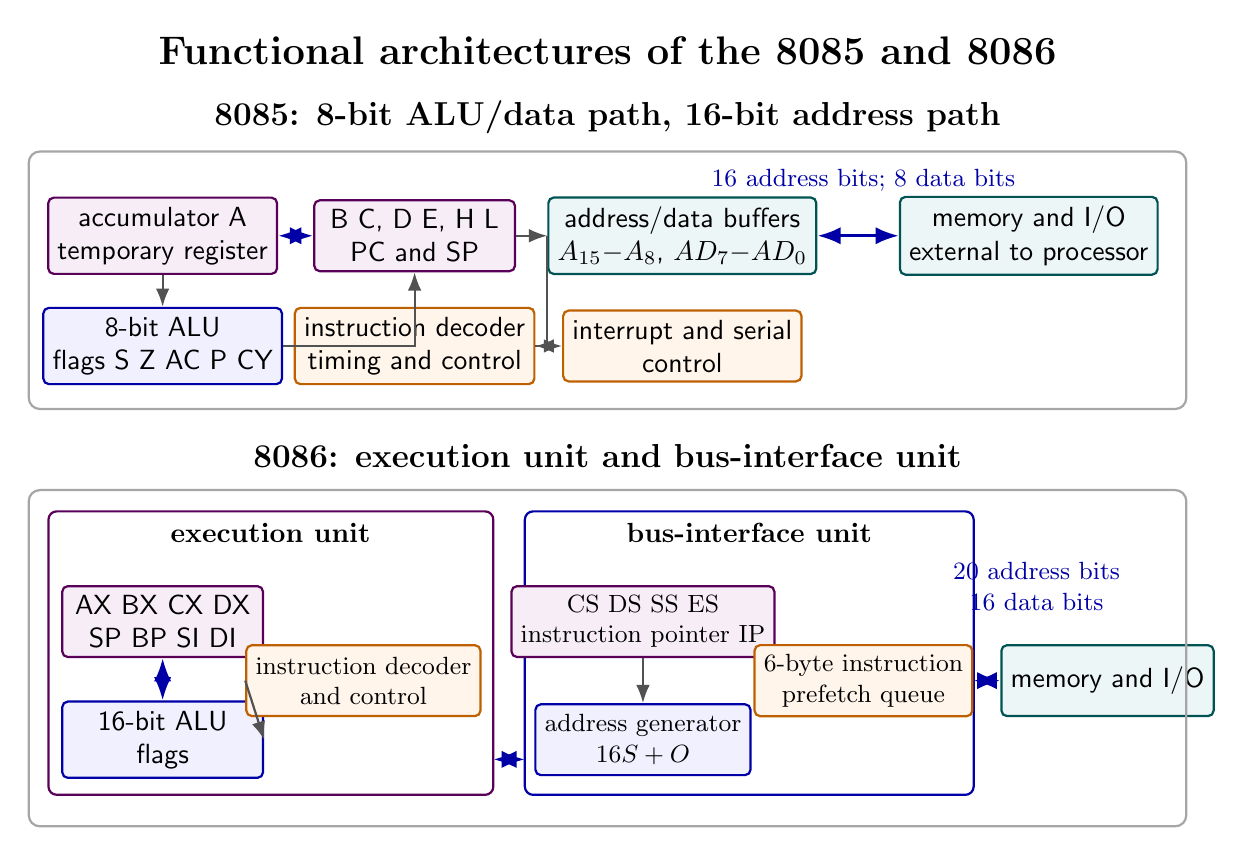
\begin{tikzpicture}[
  font=\sffamily,
  >=Latex,
  block/.style={draw=blue!65!black,rounded corners=2pt,thick,minimum width=2.55cm,minimum height=.9cm,align=center,fill=blue!6},
  reg/.style={block,draw=violet!70!black,fill=violet!7},
  ctl/.style={block,draw=orange!75!black,fill=orange!8},
  ext/.style={block,draw=teal!65!black,fill=teal!7},
  flow/.style={->,thick,black!68},
  bus/.style={<->,very thick,blue!65!black}
]
\node[font=\bfseries\Large] at (7.8,11.0) {Functional architectures of the 8085 and 8086};

% 8085: 8-bit processor path and 16-bit address interface.
\node[font=\bfseries\large] at (7.8,10.15) {8085: 8-bit ALU/data path, 16-bit address path};
\node[reg] (a85) at (2.15,8.65) {accumulator A\\temporary register};
\node[block] (alu85) at (2.15,7.25) {8-bit ALU\\flags S Z AC P CY};
\node[reg] (r85) at (5.35,8.65) {B C, D E, H L\\PC and SP};
\node[ctl,minimum width=2.85cm] (d85) at (5.35,7.25) {instruction decoder\\timing and control};
\node[ext,minimum width=3.1cm] (b85) at (8.75,8.65) {address/data buffers\\$A_{15}{-}A_8$, $AD_7{-}AD_0$};
\node[ctl,minimum width=2.85cm] (i85) at (8.75,7.25) {interrupt and serial\\control};
\node[ext,minimum width=2.8cm] (m85) at (13.15,8.65) {memory and I/O\\external to processor};
\draw[bus] (a85) -- (r85);
\draw[flow] (a85) -- (alu85);
\draw[flow] (alu85.east) -| (r85.south);
\draw[flow] (r85) -- (b85);
\draw[flow] (b85.west) |- (d85.east);
\draw[flow] (d85) -- (i85);
\draw[bus] (b85) -- (m85);
\node[font=\small,blue!65!black] at (11.05,9.35) {16 address bits; 8 data bits};
\draw[rounded corners=4pt,thick,black!35] (.45,6.45) rectangle (15.15,9.72);

% 8086: explicit non-overlapping execution and bus-interface regions.
\node[font=\bfseries\large] at (7.8,5.85) {8086: execution unit and bus-interface unit};
\draw[rounded corners=3pt,thick,violet!70!black] (.7,1.55) rectangle (6.35,5.15);
\node[font=\bfseries] at (3.52,4.88) {execution unit};
\node[reg] (regs86) at (2.15,3.75) {AX BX CX DX\\SP BP SI DI};
\node[block] (alu86) at (2.15,2.25) {16-bit ALU\\flags};
\node[ctl,font=\small,minimum width=2.45cm] (dec86) at (4.7,3.0) {instruction decoder\\and control};
\draw[bus] (regs86) -- (alu86);
\draw[flow] (dec86.west) -- (alu86.east);

\draw[rounded corners=3pt,thick,blue!65!black] (6.75,1.55) rectangle (12.45,5.15);
\node[font=\bfseries] at (9.6,4.88) {bus-interface unit};
\node[reg,font=\small,minimum width=2.65cm] (seg86) at (8.25,3.75) {CS DS SS ES\\instruction pointer IP};
\node[block,font=\small] (ag86) at (8.25,2.25) {address generator\\$16S+O$};
\node[ctl,font=\small,minimum width=2.25cm] (q86) at (11.05,3.0) {6-byte instruction\\prefetch queue};
\draw[flow] (seg86) -- (ag86);
\draw[bus] (6.35,2.0) -- (6.75,2.0);

\node[ext,minimum width=2.6cm] (m86) at (14.15,3.0) {memory and I/O};
\draw[bus] (12.45,3.0) -- (m86.west);
\node[font=\small,blue!65!black,align=center] at (13.25,4.2) {20 address bits\\16 data bits};
\draw[rounded corners=4pt,thick,black!35] (.45,1.15) rectangle (15.15,5.42);
\end{tikzpicture}
\end{document}
